\documentclass{article}
\usepackage[utf8]{inputenc}
\usepackage[italian]{babel}
\usepackage{amsmath} % extra math environments
\usepackage{graphicx} % add figures 
\usepackage{subcaption} % add subfigures
\usepackage{hyperref} % add hypertext links
\usepackage{minted} % add code snippets
\usepackage{siunitx} % SI units formatting

\title{Relazione di Laboratorio 1 - Catenaria}
\author{Walhout Francesco - Iallorenzi Michele}
\date{28 Ottobre 2021}

% Color setup for hyperref
\hypersetup{
    colorlinks=true,
    linkcolor=cyan,
    urlcolor=blue
    }

\begin{document}

\maketitle

\section{Introduzione}
La catenaria è una funzione che descrive l'andamento di una fune omogenea, 
flessibile e non estensibile, i cui due estremi sono fissati e che viene lasciata pendere,
soggetta ad un campo gravitazionale.
In questa esperienza di Laboratorio cercheremo di dimostrare che la funzione
catenaria risulta essere una buona approssimazione di una catena reale lasciata appesa
per i suoi estremi.\\
La funzione della catenaria è la seguente:

\begin{equation}
    \label{eq:catenaria}
    f(x) = y_0 + a \cdot \cosh(\frac{x-x_0}{a})
\end{equation}

\subsection{Strumenti utilizzati}
\begin{itemize}
    \item Una catena di una collana.
    \item Righello o metro a nastro.
    \item Smartphone o macchina fotografica digitale.
    \item Carta millimetrata.
    \item Nastro adesivo.
\end{itemize}

\section{Misure ed analisi}

\subsection{Preparazione}
Per prima cosa bisogna organizzare la carta millimetrata.
Useremo una catena di una collana che risulta essere:
molto flessibile,
adatta a calcolare l'incertezza di misura (come vedremo dopo)
e di una grandezza giusta per poter entrare nel foglio.
Bisognerà prendere la collana e porre i due capi il più allineati possibile,
ad una certa distanza scelta arbitrariamente;
a questo scopo ci siamo aiutati cercando di fissare, a matita,
due punti dove si dovrà iniziare la misurazione.
Una volta scelti i punti si cerca di fissare, con del nastro adesivo, la catena,
in modo tale che si sovrapponga ai punti che abbiamo già segnato,
nella presa dati ignoreremo la parte della catena al di sopra di questi ultimi
(quindi molto vicina ai punti di fissaggio) poiché 
il nastro adesivo potrebbe modificare la forma della collana.
Questo è il risultato finale:

\begin{figure}[ht]
    \centering
    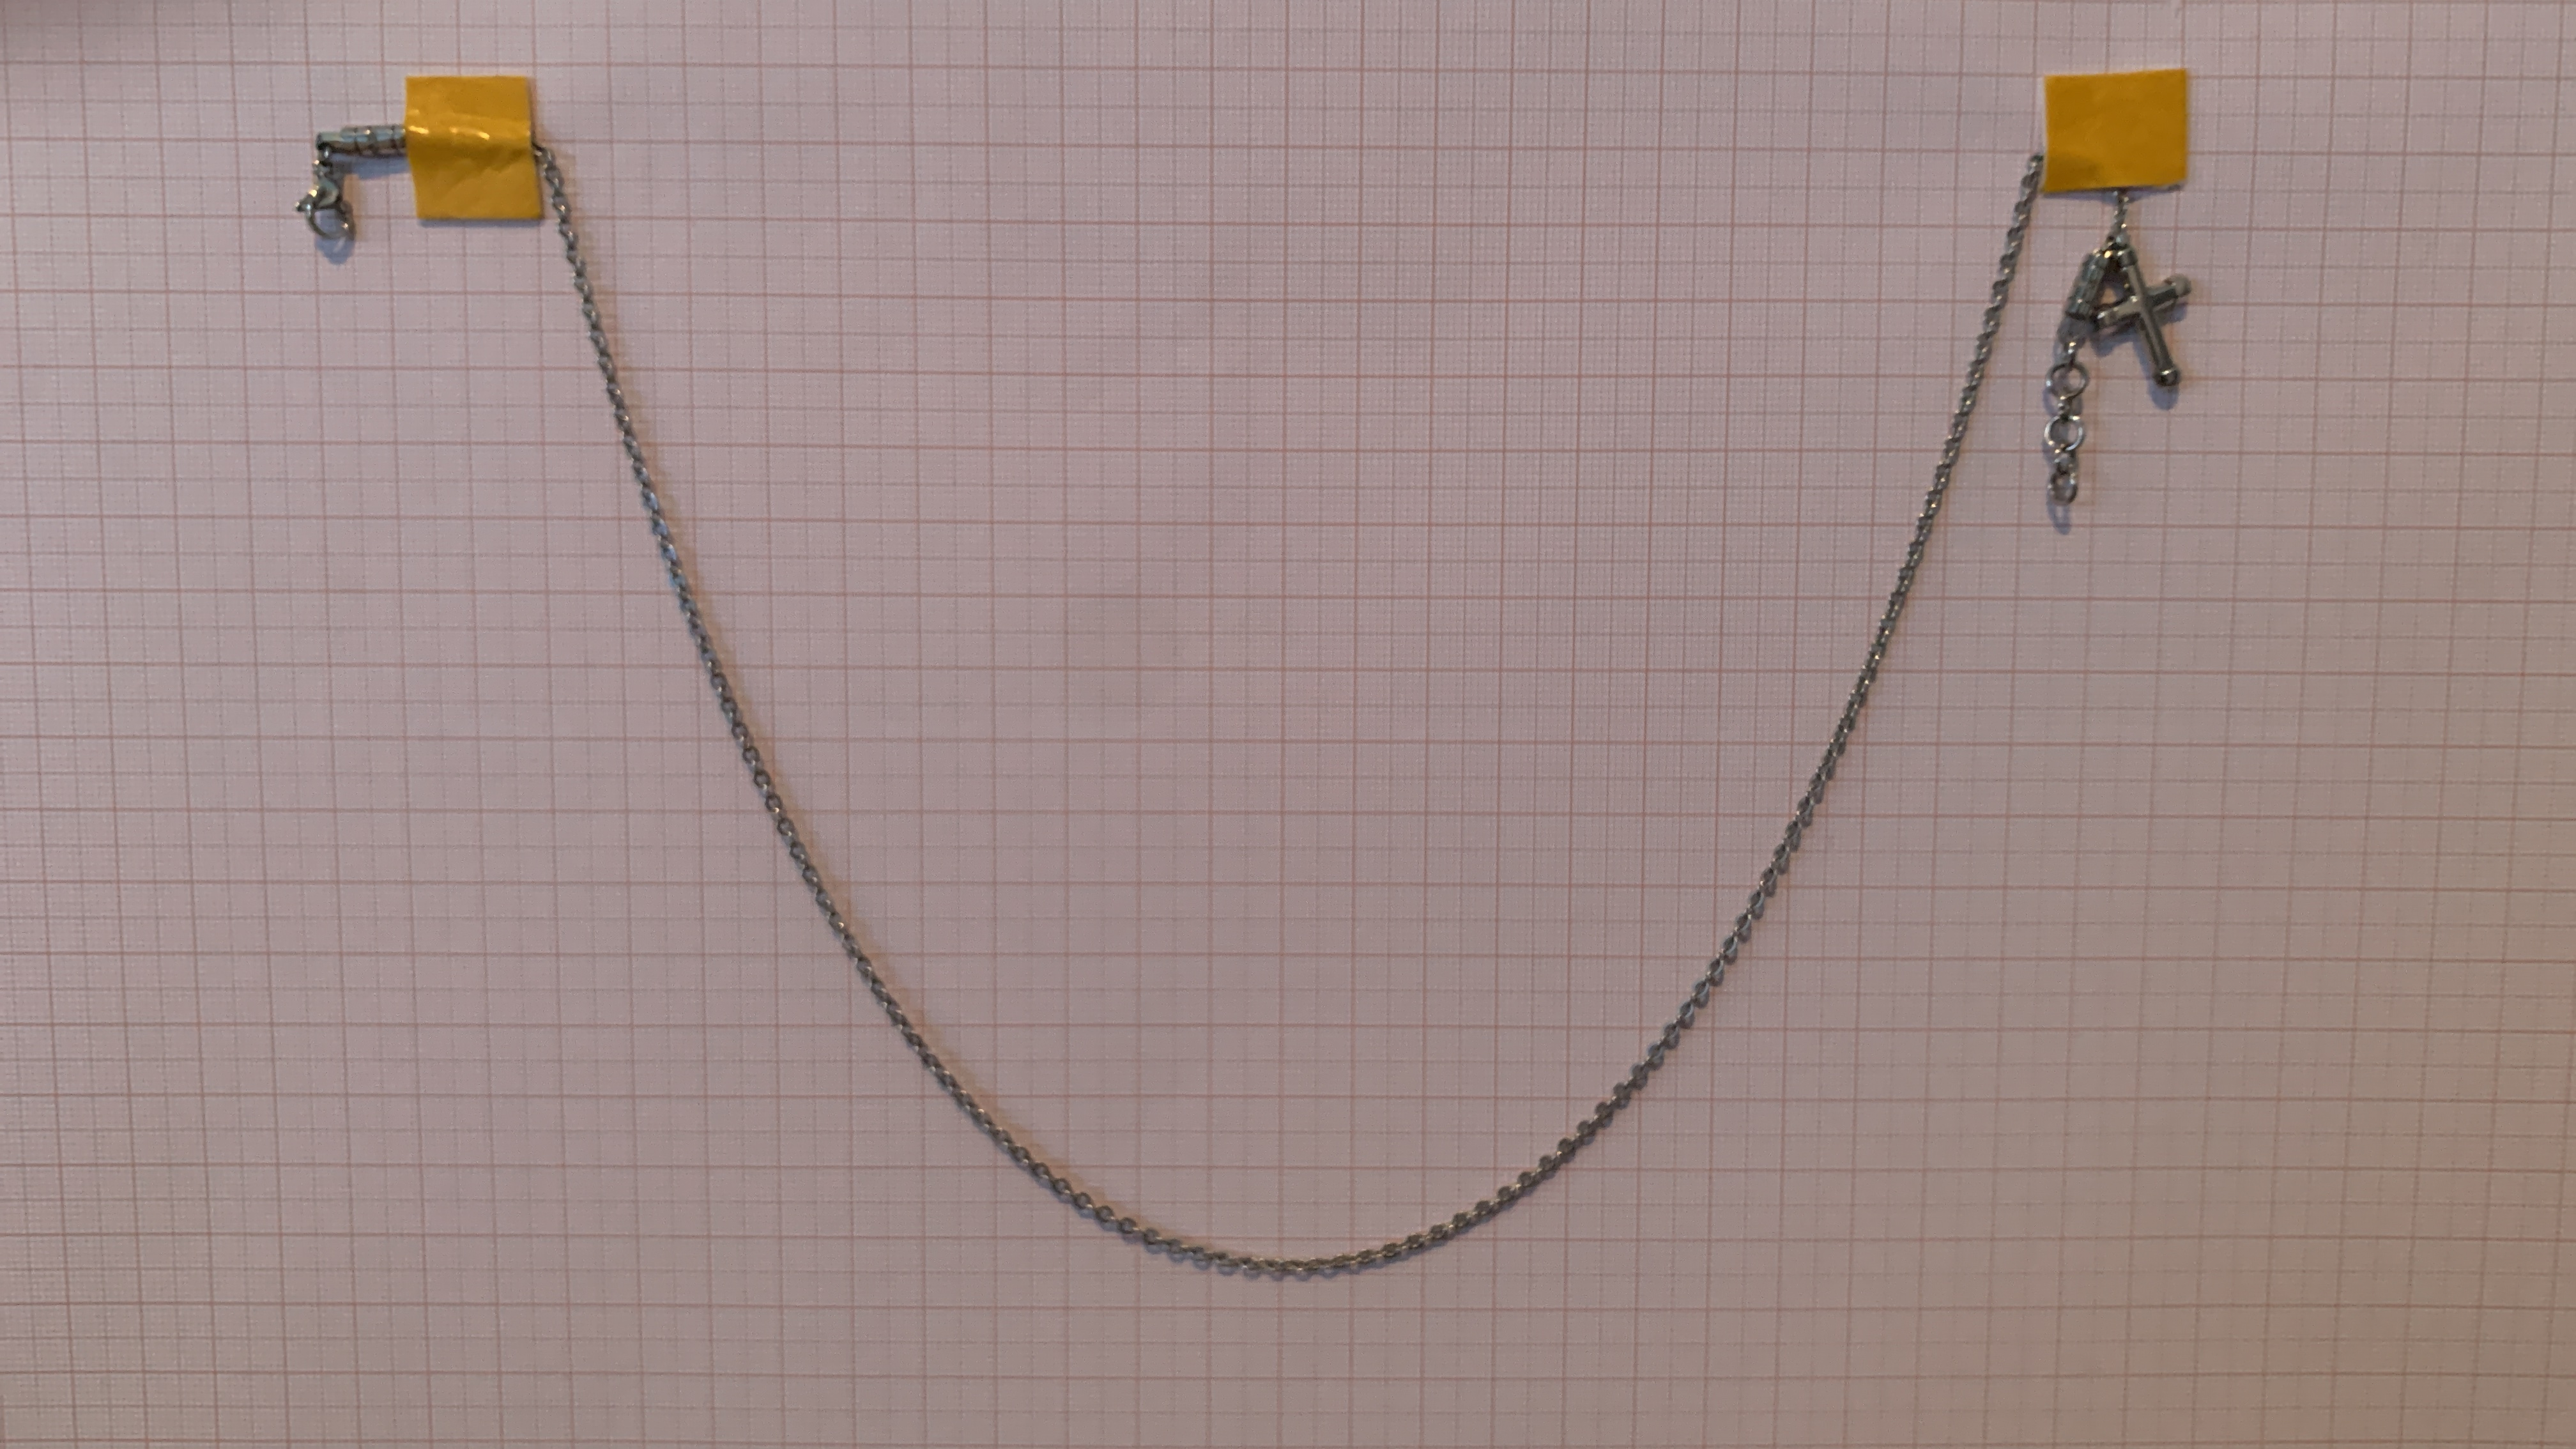
\includegraphics[width=0.8\textwidth]{extra/catenaria_immagine.jpg}
    \caption{Foto del setup sperimentale da cui sono stati estratti i dati dell'esperienza.}
    \label{fig:my_label}
\end{figure}

Per poter ottenere l'andamento della catenaria che ci interessa,
dovremo attaccare al muro il foglio, in questo modo la forza peso sarà esercitata
in ogni punto della catena.
Per scattare la foto abbiamo cercato di porre lo smartphone più parallelamente possibile
al muro aiutandoci con una livella ed un treppiede.

\subsection{Misurazione}
La misurazione è stata fatta sfruttando la piattaforma \href{https://automeris.io/WebPlotDigitizer/}{WebPlotDigitizer},
dove è possibile caricare la propria foto,
fissare degli assi $x$ ed $y$ e prendere le misure nella stessa foto,
cercando di inserire (nel modo più preciso possibile) una serie di punti nel piano.
L'unità che abbiamo scelto è il centimetro, poiché grazie alla carta millimetrata che fa da
riferimento WebPlotDigitizer permette di ottenere misure direttamente in centimetri.
Per la misurazione abbiamo cercato di prendere i punti il più possibile al centro di ciascun anello
in modo tale che i valori riportati non si distacchino dal misurando di più di metà dello
spessore della catena.
Questo significa che, una trovato il diametro dell'anello,
si ottiene anche un margine di errore per le misure,
nel mio caso ho avuto un margine di errore di:

\begin{gather*}
    d = \SI{0.20}{\cm} \\
    D = \SI{0.25}{\cm}
\end{gather*}

dove $d$ è il diametro minore dell'anello e $D$ è quello maggiore.
L'incertezza di misura sarà data da metà del diametro maggiore dell'anello:
\begin{equation*}
    \sigma = \SI{.12}{\cm}
\end{equation*}

\section{Elaborazione dei dati}
Questa parte è dedicata alla programmazione di un software che permetta
di raccogliere tutti i punti trovati nel piano per poi sistemarli in un grafico
(con assi $x$ [cm] ed $y$ [cm]), tutto nel linguaggio di programmazione Python.
Il programma utilizza la funzione \href{https://docs.scipy.org/doc/scipy/reference/generated/scipy.optimize.curve_fit.html}{curve\_fit}
della libreria scipy per eseguire il fit dei dati e quindi determinare per quali
parametri la funzione \ref{eq:catenaria} rappresenta meglio i dati sperimentali.\\
Infine il codice inserisce un grafico dei residui i cui valori equivalgono alla differenza
tra i valori sperimentali e quelli della funzione catenaria trovata attraverso il fit.
Le librerie utilizzare sono numpy, matplotlib e scipy. Il codice sorgente è il seguente:
\inputminted[linenos, frame=single]{python}{extra/catenaria.py}

\section{Conclusioni}
\begin{figure}[ht]
    \centering
    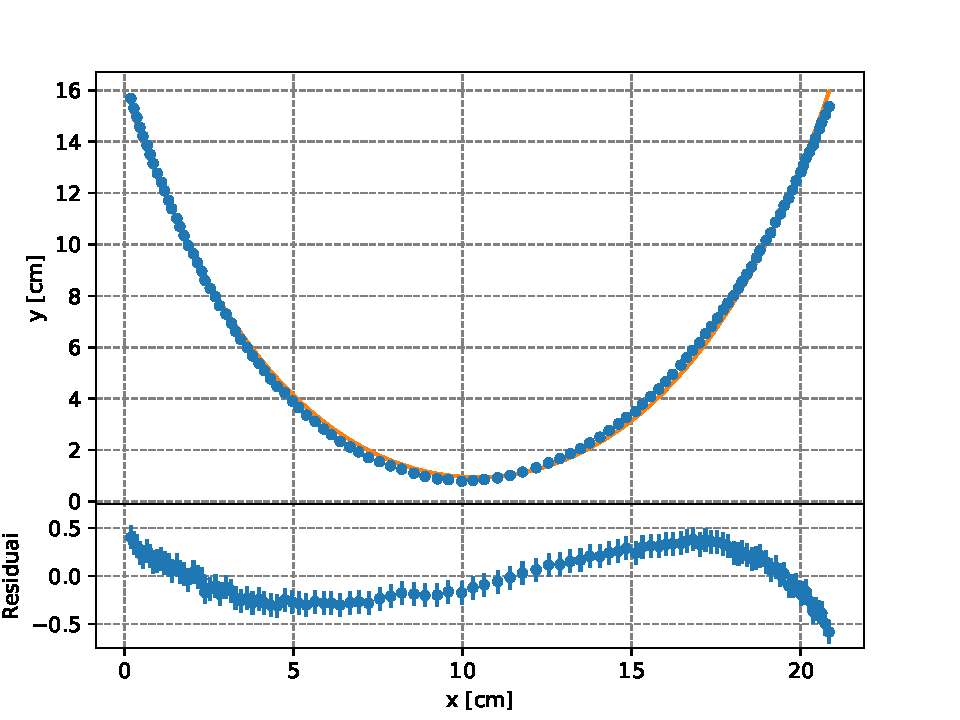
\includegraphics[width=0.8\textwidth]{extra/catenaria.pdf}
    \caption{Risultato dell'elaborazione attraverso lo script in python}
    \label{fig:extra-catenaria-pdf}
\end{figure}
Nel grafico ottenuto è possibile notare ad occhio che la funzione catenaria segue effettivamente
l'andamento delle misure, ma osservando il grafico dei residui si nota
che è presente un errore non trascurabile in quanto i valori si distaccano notevolmente dallo zero.
Quindi la funzione vista prima è una buona ma non perfetta approssimazione dell'andamento
di una catena reale.

\section{Interessanti applicazioni}
Queste nozioni che sono state apprese, ci sono estremamente utili per poter ri-
flettere su alcuni aspetti architettonici, infatti questa curva è estremamente utile
per costruire ponti, cupole e archi. Come abbiamo visto, una qualsiasi catena
si dispone in questo modo per via della forza peso esercitata su di essa, in par-
ticolare, la catenaria che si forma, ha la proprietà di avere in ogni suo punto
una distribuzione uniforme del suo peso totale. Sfruttando questa proprietà (e
conoscendo la funzione che descrive la curva) è stato possibile creare delle strut-
ture architettoniche come il ponte ferroviario Garabit (Gustave Eiffel), il Gateway Arch a 
St. Louis (Eero Saarinen) o la Cupola di St. Paul a Londra (Sir Christopher
Wren), infatti in queste opere architettoniche sono presenti degli archi che descrivono
una catenaria e che riescono quindi a distribuire il peso.
\begin{figure}[h!]
    \centering
    \begin{subfigure}[b]{0.3\linewidth}
        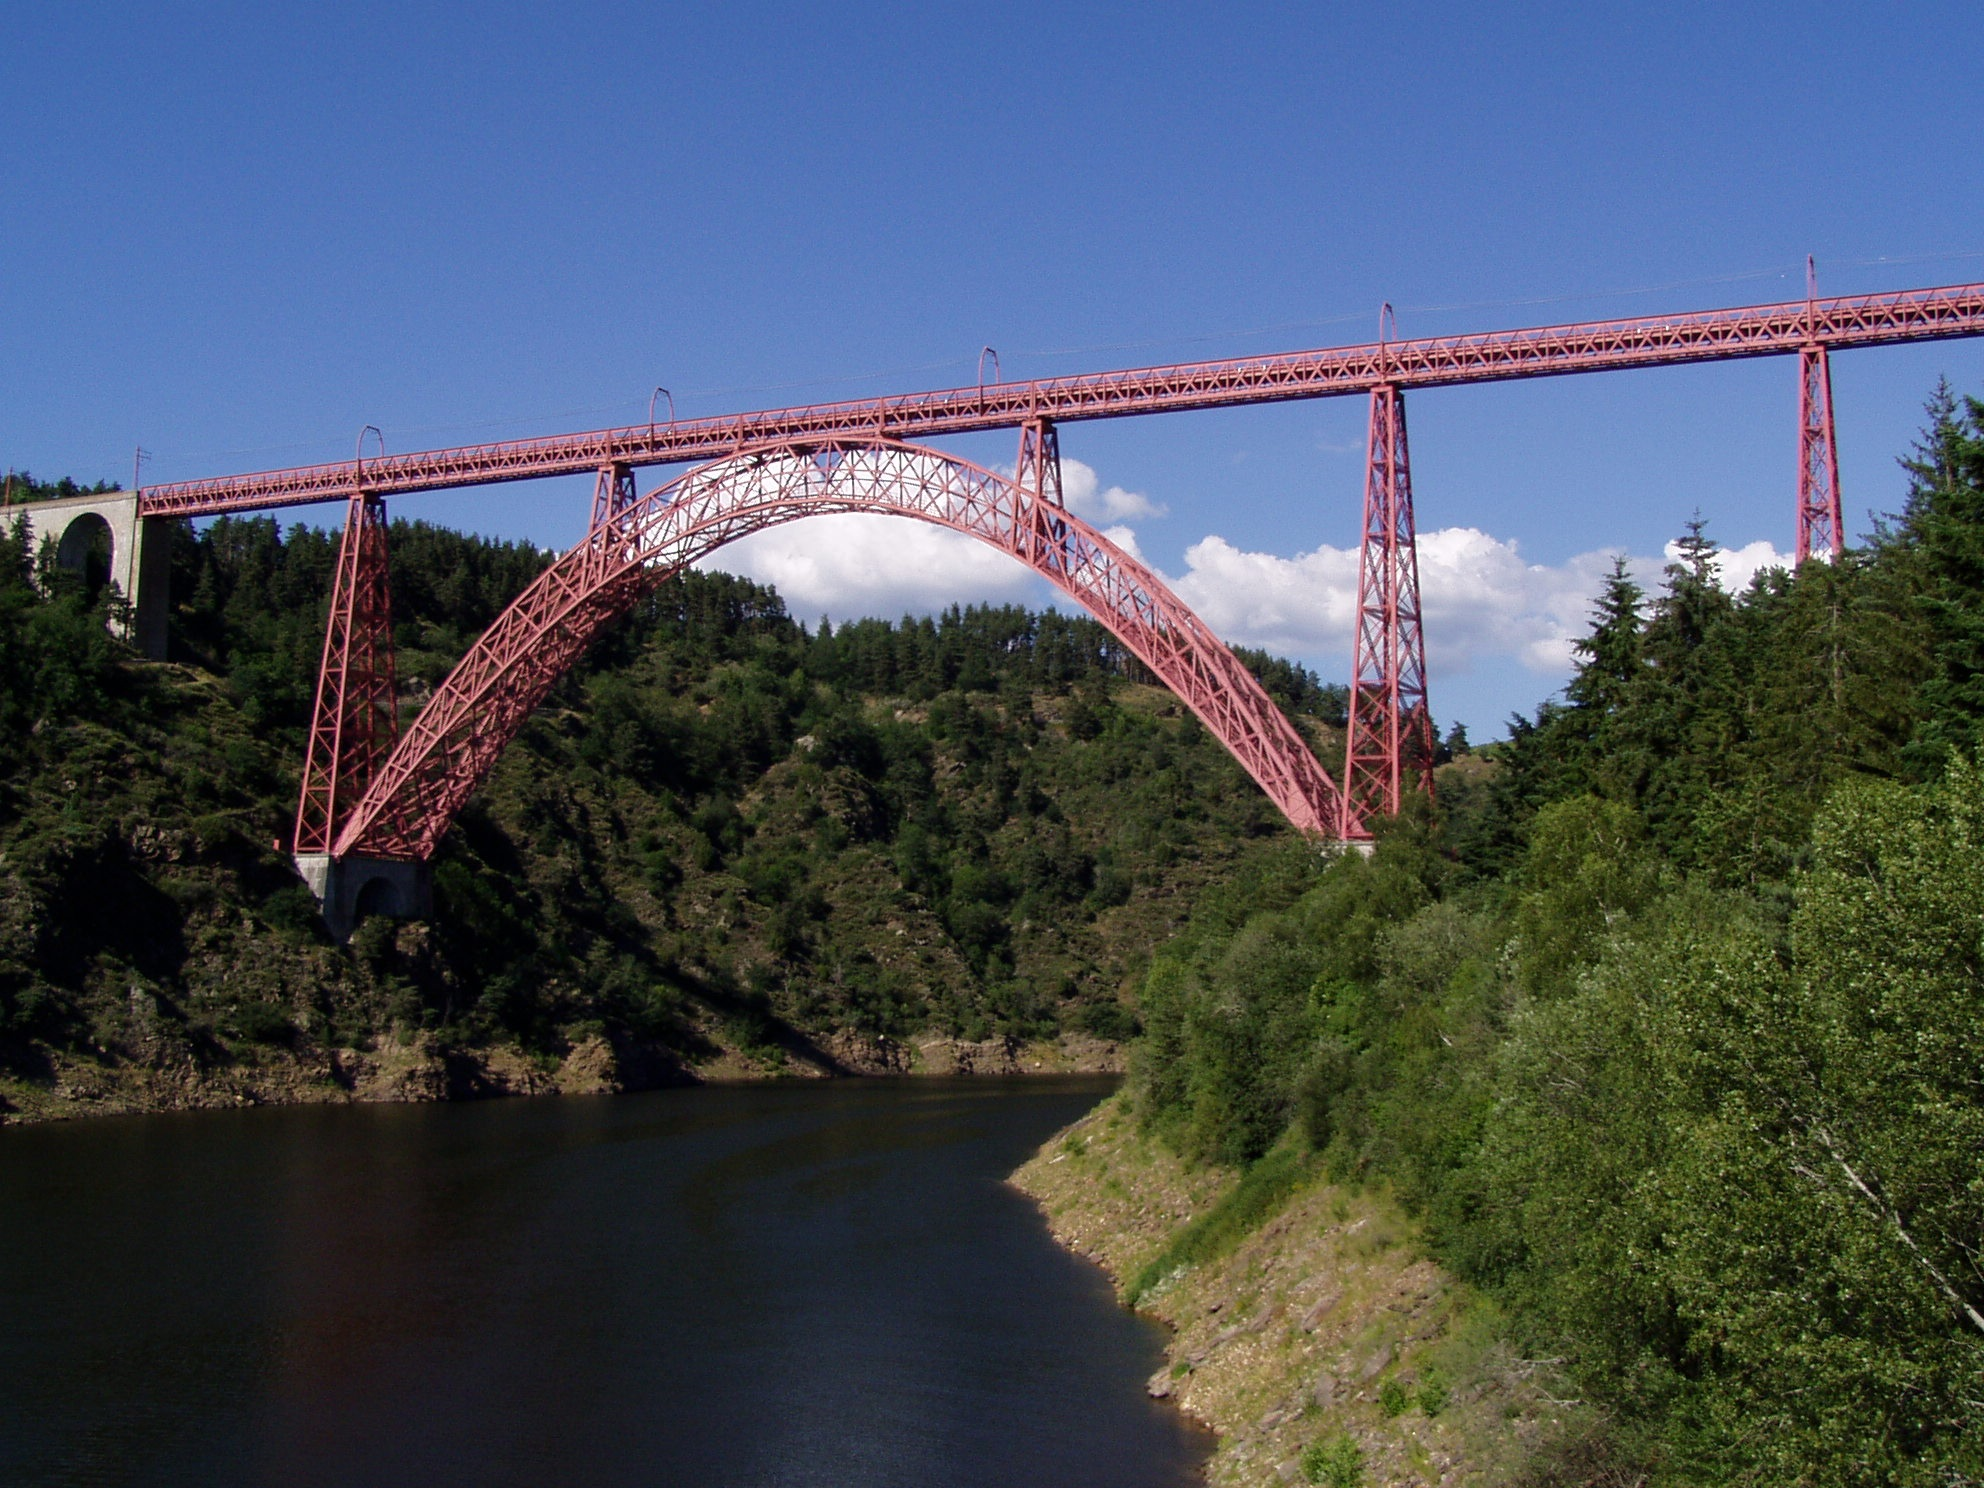
\includegraphics[width=\linewidth]{extra/viadotto_di_garabit.jpg} 
    \end{subfigure}
    \begin{subfigure}[b]{0.3\linewidth}
        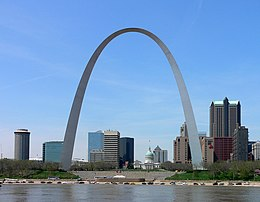
\includegraphics[width=\linewidth]{extra/st_louis_arco.jpg} 
    \end{subfigure}
    \begin{subfigure}[b]{0.3\linewidth}
        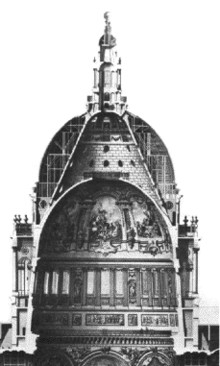
\includegraphics[width=\linewidth]{extra/cupola_cattedrale_san_paolo.jpg} 
    \end{subfigure}
    \caption{Da sinistra verso destra: \emph{viadotto di Garabit}, Ruynes-en-Margeride, Francia, Gustave Eiffel; \emph{Gateway Arch}, St. Louis, Stati Uniti, Eero Saarinen; cupola della \emph{cattedrale di San Paolo}, Londra, Regno unito, Christopher Wren.}
    \label{fig:applicazioni}
\end{figure}

\end{document}
